\section{Rigid body kinematics}

Describe the coordinate systems.

Following the notation presented in \cite{kiencke} we will employ a 4 main coordinate systems, summarized in the list below.
\begin{itemize}
    \item $CG$ for the chassis (Center of Gravity) coordinate system,
    \item $Un$ for the undercarriage system,
    \item $W$ for the wheel coordinate systems,
    \item $In$ for the fixed inertial system.
\end{itemize}

\info[inline]{For controlling it might be useful to define a tool coordinate system as well.}
\improve[inline]{Not clear whether CG system should be defined with or without weight of tools.}
\improve[inline]{The CG is not a center of rotation. Might need an additional point to describe center of rotation. See how the single track model solves this.}

The inertial system $In$ has a fixed origin and is the only coordinate system that doesn't move during travel. To describe the pose, that is position and orientation, of the vehicle we will use a coordinate system placed in the center of gravity, denoted $CG$. The orientation of the $CG$ system is with the x-axis pointing out the front of the vehicle. 
It will be useful to have an undercarriage coordinate system $Un$. This has the same orientation as the $CG$ system, but it has it's origin perpendicular to the rear axle in the midpoint between the rear wheels at road level. Each wheel is also given a coordinate system $Wij$ in the center of each wheel with the x-axis pointing in the wheel forward direction and z-axis aligned with the undercarriage z-axis. These coordinate systems are illustrated in \cref{fig:coords-side,fig:coords-top}. 

\begin{figure}
    \centering
    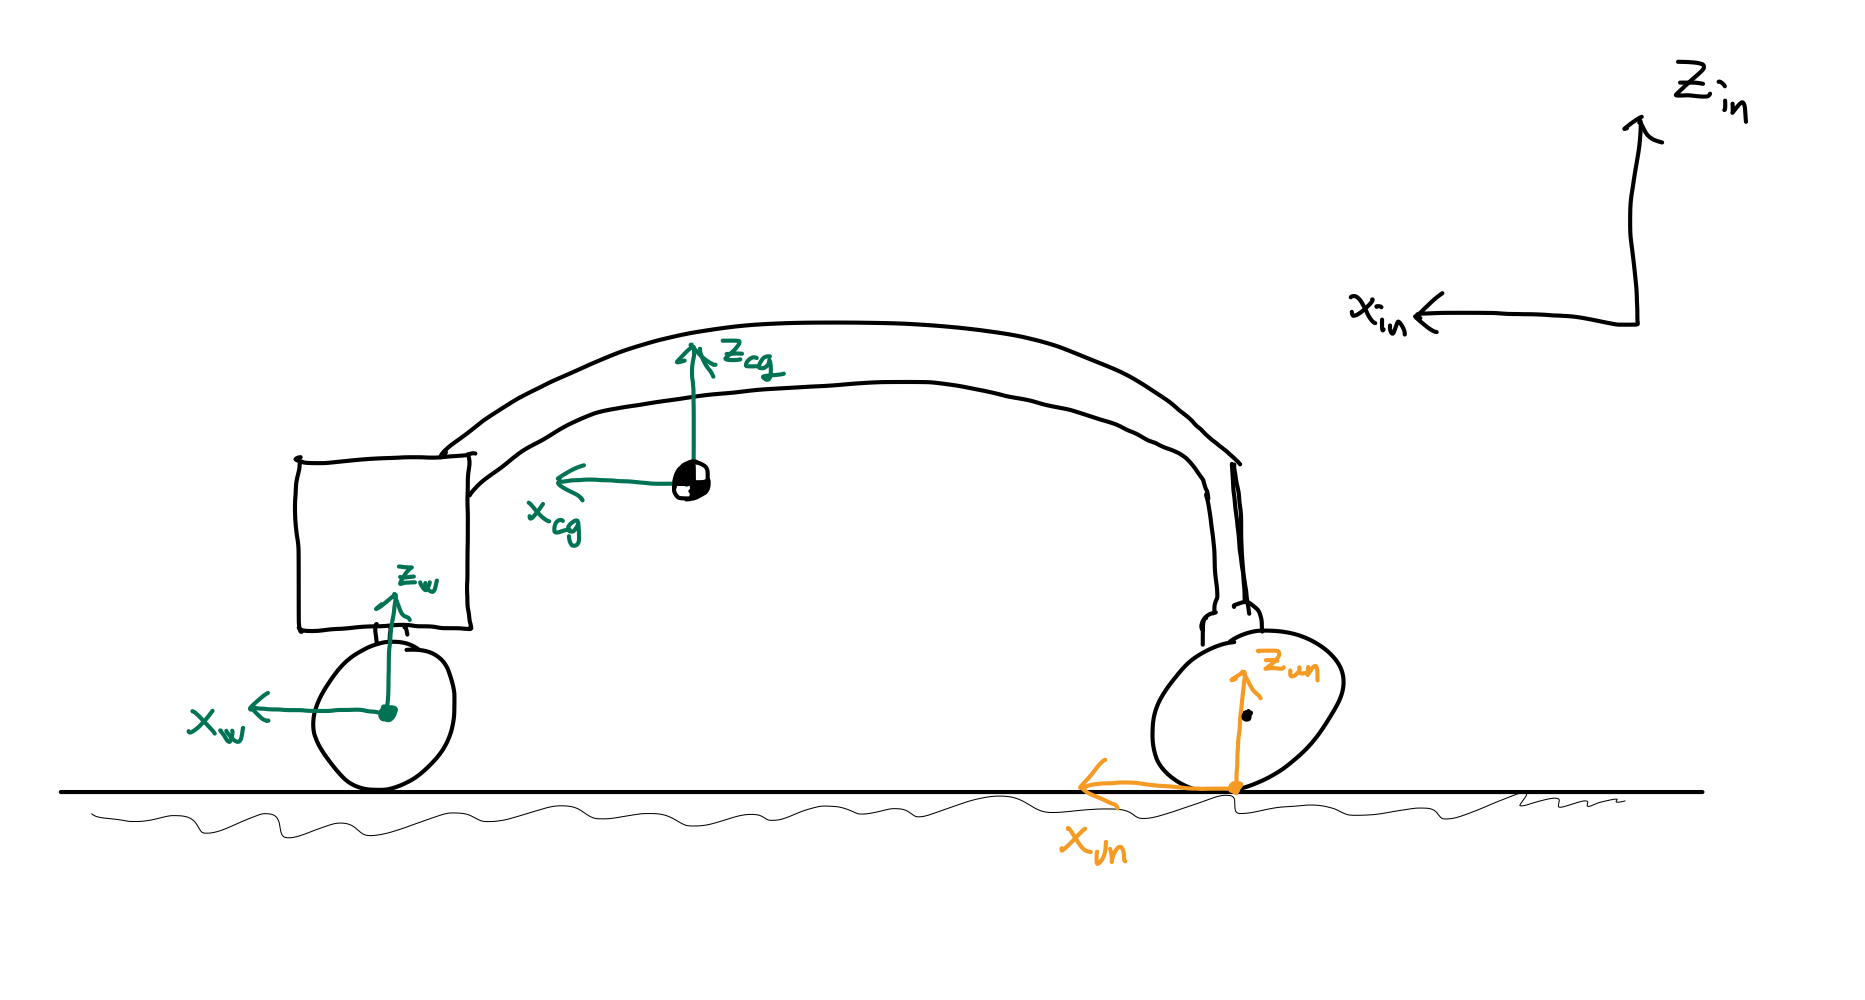
\includegraphics[width=\textwidth]{sections/figures/side-coordinate-systems-sketch.jpeg}
    \caption{Coordinate systems viewed from side}
    \label{fig:coords-side}
\end{figure}

\begin{figure}
    \centering
    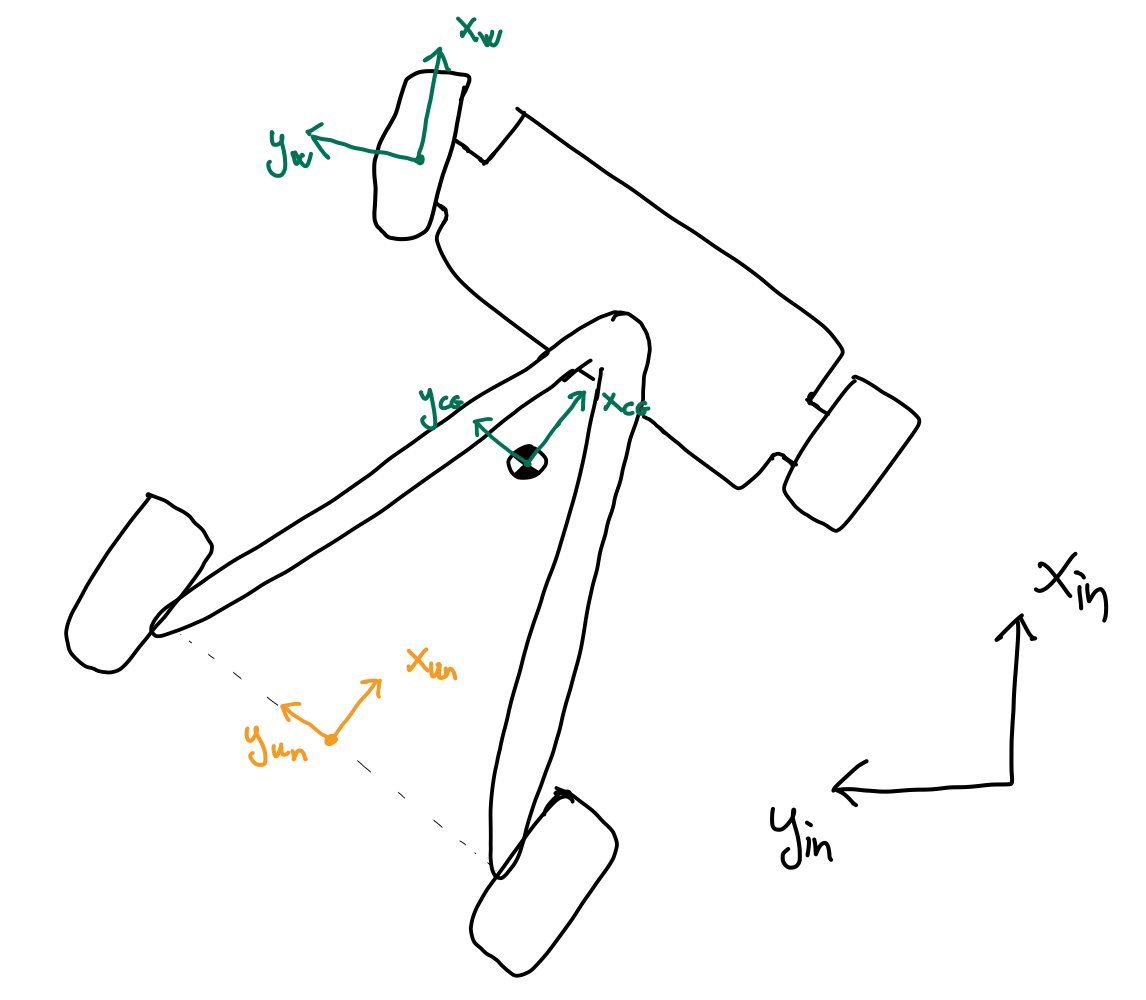
\includegraphics[width=\textwidth]{sections/figures/top-coordinate-systems-sketch.jpeg}
    \caption{Coordinate systems viewed from top}
    \label{fig:coords-top}
\end{figure}

We will now define the transforms needed to do computations on these coordinate systems. The transform tree we will use is given in \cref{fig:transform-tree}. The dotted arrow is a constant transform whereas the solid arrows change over time.

\begin{figure}
    \centering
    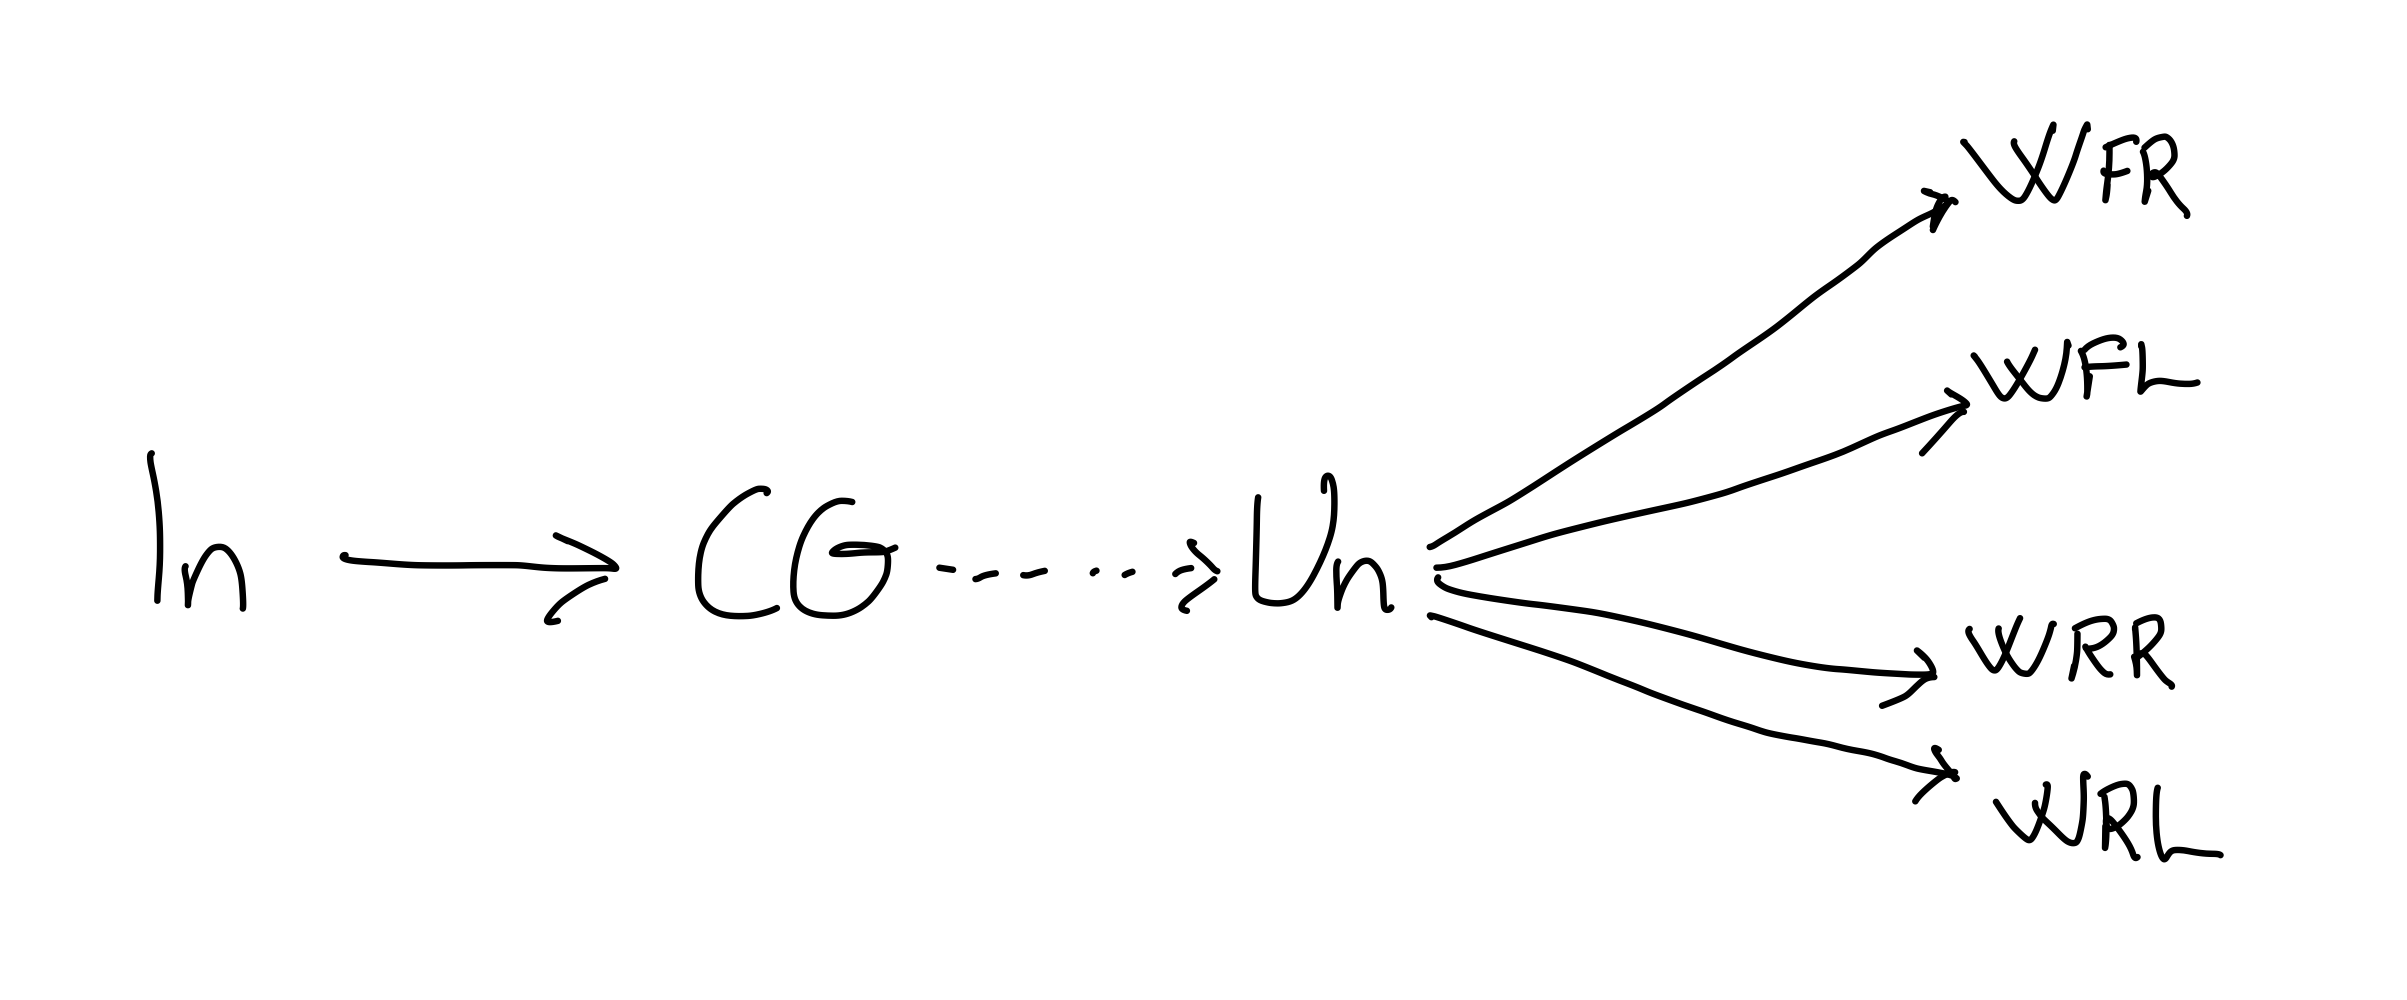
\includegraphics[width=\textwidth]{sections/figures/coordinate-tree.jpeg}
    \caption{Coordinate systems connections}
    \label{fig:transform-tree}
\end{figure}


To denote the position of the vehicle we will use $x,y,z$ which is the position of the center of gravity in the $In$ system.


\begin{equation}
  \mathbf{T}_{CG}^{In} = 
  \begin{bmatrix}
    \mathbf{R}_{CG}^{In} & \mathbf{o}_{CG}^{In} \\
    \mathbf{0} & 1
  \end{bmatrix}
  =
  \begin{bmatrix}
    ? & ? & ? & x \\
    ? & ? & ? & y \\
    ? & ? & ? & z \\
    0 & 0 & 0 & 1
  \end{bmatrix}
\end{equation}

\todo[inline]{review chapter from Modelling and Control of Robots to get a handle on these rotation matrices.}


Let $L_r$ be the distance from CG to the rear axle along the x-axis in $CG$ and the $h_{CG}$ the distance from the CG to the ground along the z-axis in $CG$. 
With these constants then the undercarriage system is defined as a pure translation of the $CG$ system.

\begin{equation}
  \mathbf{T}_{Un}^{CG} = 
  \begin{bmatrix}
    \mathbf{I} & \mathbf{o}_{Un}^{CG} \\
    \mathbf{0} & 1
  \end{bmatrix}
  =
  \begin{bmatrix}
    1 & 0 & 0 & -L_r \\
    0 & 1 & 0 & 0 \\
    0 & 0 & 1 & -h_{CG} \\
    0 & 0 & 0 & 1
  \end{bmatrix}
\end{equation}


Let $L_f$ be the distance from CG to the front axle along the x-axis in $CG$, $r_W$ be the radius of the wheels, $B_f$ be the distance between the front wheels, and $B_r$ be the distance between the rear wheels. In addition each wheel is rotated be some angle $\delta_{Wij}$ around the z-axis. From these parameters we can define all four wheel coordinate systems.


\begin{align}
  \mathbf{T}_{WFL}^{Un} &= 
  \begin{bmatrix}
    \mathbf{R}_z(\pm \delta_{WFL}) & \mathbf{o}_{WFL}^{Un} \\
    \mathbf{0} & 1
  \end{bmatrix}
  =
  \begin{bmatrix}
    ? & ? & 0 & L_r + L_f \\
    ? & ? & 0 & B_f/2 \\
    0 & 0 & 1 & r_W \\
    0 & 0 & 0 & 1
  \end{bmatrix} \\
  \mathbf{T}_{WFR}^{Un} &= 
  \begin{bmatrix}
    \mathbf{R}_z(\pm \delta_{WFR}) & \mathbf{o}_{WFR}^{Un} \\
    \mathbf{0} & 1
  \end{bmatrix}
  =
  \begin{bmatrix}
    ? & ? & 0 & L_r + L_f \\
    ? & ? & 0 & -B_f/2 \\
    0 & 0 & 1 & r_W \\
    0 & 0 & 0 & 1
  \end{bmatrix} \\
  \mathbf{T}_{WRL}^{Un} &= 
  \begin{bmatrix}
    \mathbf{R}_z(\pm \delta_{WRL}) & \mathbf{o}_{WRL}^{Un} \\
    \mathbf{0} & 1
  \end{bmatrix}
  =
  \begin{bmatrix}
    ? & ? & 0 & 0 \\
    ? & ? & 0 & B_r/2 \\
    0 & 0 & 1 & r_W \\
    0 & 0 & 0 & 1
  \end{bmatrix} \\
  \mathbf{T}_{WRR}^{Un} &= 
  \begin{bmatrix}
    \mathbf{R}_z(\pm \delta_{WRR}) & \mathbf{o}_{WRR}^{Un} \\
    \mathbf{0} & 1
  \end{bmatrix}
  =
  \begin{bmatrix}
    ? & ? & 0 & 0 \\
    ? & ? & 0 & -B_r/2 \\
    0 & 0 & 1 & r_W \\
    0 & 0 & 0 & 1
  \end{bmatrix} \\
\end{align}









